\section{Physical properties}
The phase space variables can be used to sample statistical properties of the system. Properties of interest are kinetic and potential energy, temperature, pressure, diffusion constant and different correlation functions (such as the pair correlation function, cage-correlation function, static and the dynamic structure factor). In this section, we will define these properties and discuss how to measure them.
\subsection{Kinetic and potential energy}
We measure the kinetic energy directly through its definition for point particles
\begin{align}
	E_k = \sum_i \frac{1}{2} m_iv_i^2,
\end{align}
where $m_i$ is the mass of particle $i$ and $v_i$ is the velocity of the particle. The potential energy is measured by evaluating \eqref{eq:md_potential_energy}. We define temperature by applying the equipartition theorem using the momentum degrees of freedom
\begin{align*}
	E_k = \frac{f}{2}kT,
\end{align*}
where $f=3N$ are the three momentum variables per particle, $T$ is the temperature and $k$ is Boltzmann's constant. Solving the equation for the temperature yields
\begin{align}
	T = \frac{2E_k}{3Nk},
\end{align}
which is how we \textit{define} temperature in this model. 
\subsection{Pressure}
We will derive an expression for the pressure by using Clausius' virial function
\begin{align}
    W(\textbf{r}) = \sum_{i=1}^N \vec r_i \cdot \vec F_i^{TOT},
\end{align}
where $\vec F_i^{TOT}$ is the total force acting on atom $i$, including external forces. We assume equilibrium, so that the kinetic energy has reached an approximately constant value. We measure the statistical average of $W$ by calculating
\begin{align}
    \langle W \rangle &= \lim_{t\rightarrow\infty} {1\over t} \int_0^t d\tau \sum_{i=1}^N \vec r_i(\tau) \cdot m_i \vec{\ddot r}_i(\tau).
\end{align}
Integrating by parts gives
\begin{align}
    \label{eq:virial_and_equi}
    \langle W \rangle &= -\lim_{t\rightarrow\infty} {1\over t} \int_0^t d\tau \sum_{i=1}^N m_i |\vec{\dot r}_i(\tau)|^2 = -2E_k = -3Nk_bT,
\end{align}
by again using equipartition. Now, assume that the atoms live inside a parallelepipedic container of size $L_x, L_y, Lz$ with hard walls, with origo in one of its corners. If we divide the force into external and interatomic forces, $\vec F_i^{TOT} = \vec F_i + \vec F_i^{EXT}$, and assume that the external forces are forces from the container (no gravity or electric fields), we can calculate $W^{EXT}$. The atoms near the walls apply a pressure on the wall $P = F/A$. As an example, we look at all the atoms that are near the wall located at $x=L_x$. The virial function gives
\begin{align}
    W^{EXT}_x = \sum_{n=1}^{N_x}\vec r_n\cdot \vec F_n^{EXT},
\end{align}
where $n$ now sums over all atoms that are near the container wall at $x=L_x$. The position vectors are $\vec r_n = (L_x, y_n, z_n)$ and the force only has a component normal to the wall $F_n^{EXT} = 1/N_x(-PL_yL_z, 0, 0)$. We then get
\begin{align}
    W^{EXT}_x = -L_xPL_yL_z = -PV,
\end{align}
and by doing the same for the other dimensions, we get
\begin{align}
    W = -3PV.
\end{align}
Inserting this result into \eqref{eq:virial_and_equi} yields
\begin{align}
    \left\langle \sum_{i=1}^N \vec r_i \cdot \vec F_i\right\rangle - 3PV = -3Nk_bT
\end{align}
which can be rearranged to
\begin{align}
    PV = Nk_bT - \frac{1}{3}\left\langle \sum_{i=1}^N \vec r_i \cdot \vec F_i\right\rangle.
\end{align}
Using this result, we can define the pressure
\begin{align}
    \label{eq:pressure_in_md}
	P = \rho_n k_bT - \frac{1}{3V}\left\langle \sum_{i=1}^N \vec r_i \cdot \vec F_i\right\rangle,
\end{align}
where $\rho$ is the density.
\subsection{Radial distribution function $g(r)$}
The thermodynamic properties like temperature, pressure and volume give little or no information about the microscopic structure of the system. If the atoms forms a solid and are organized in some sort of a crystal (see figure \ref{fig:crystal}), one could be interested in measuring what kind of crystal they form. Different structures and symmetries of the crystal give rise to different physical properties like electronic band structure, optical transparency among others\cite{kittel1996introduction}. The crystal structure can be studied through what is called the radial distribution function, $g(r)$, which is a function proportional to the probability of finding an atom at a distance $r$ from another atom. A non-perfect FCC lattice (non-perfect in the sense that the atoms are vibrating around the equilibrium) will have a $g(r)$ as in figure \ref{fig:fcc_lattice_g_of_r}.\\
\begin{figure}[h]
\framebox{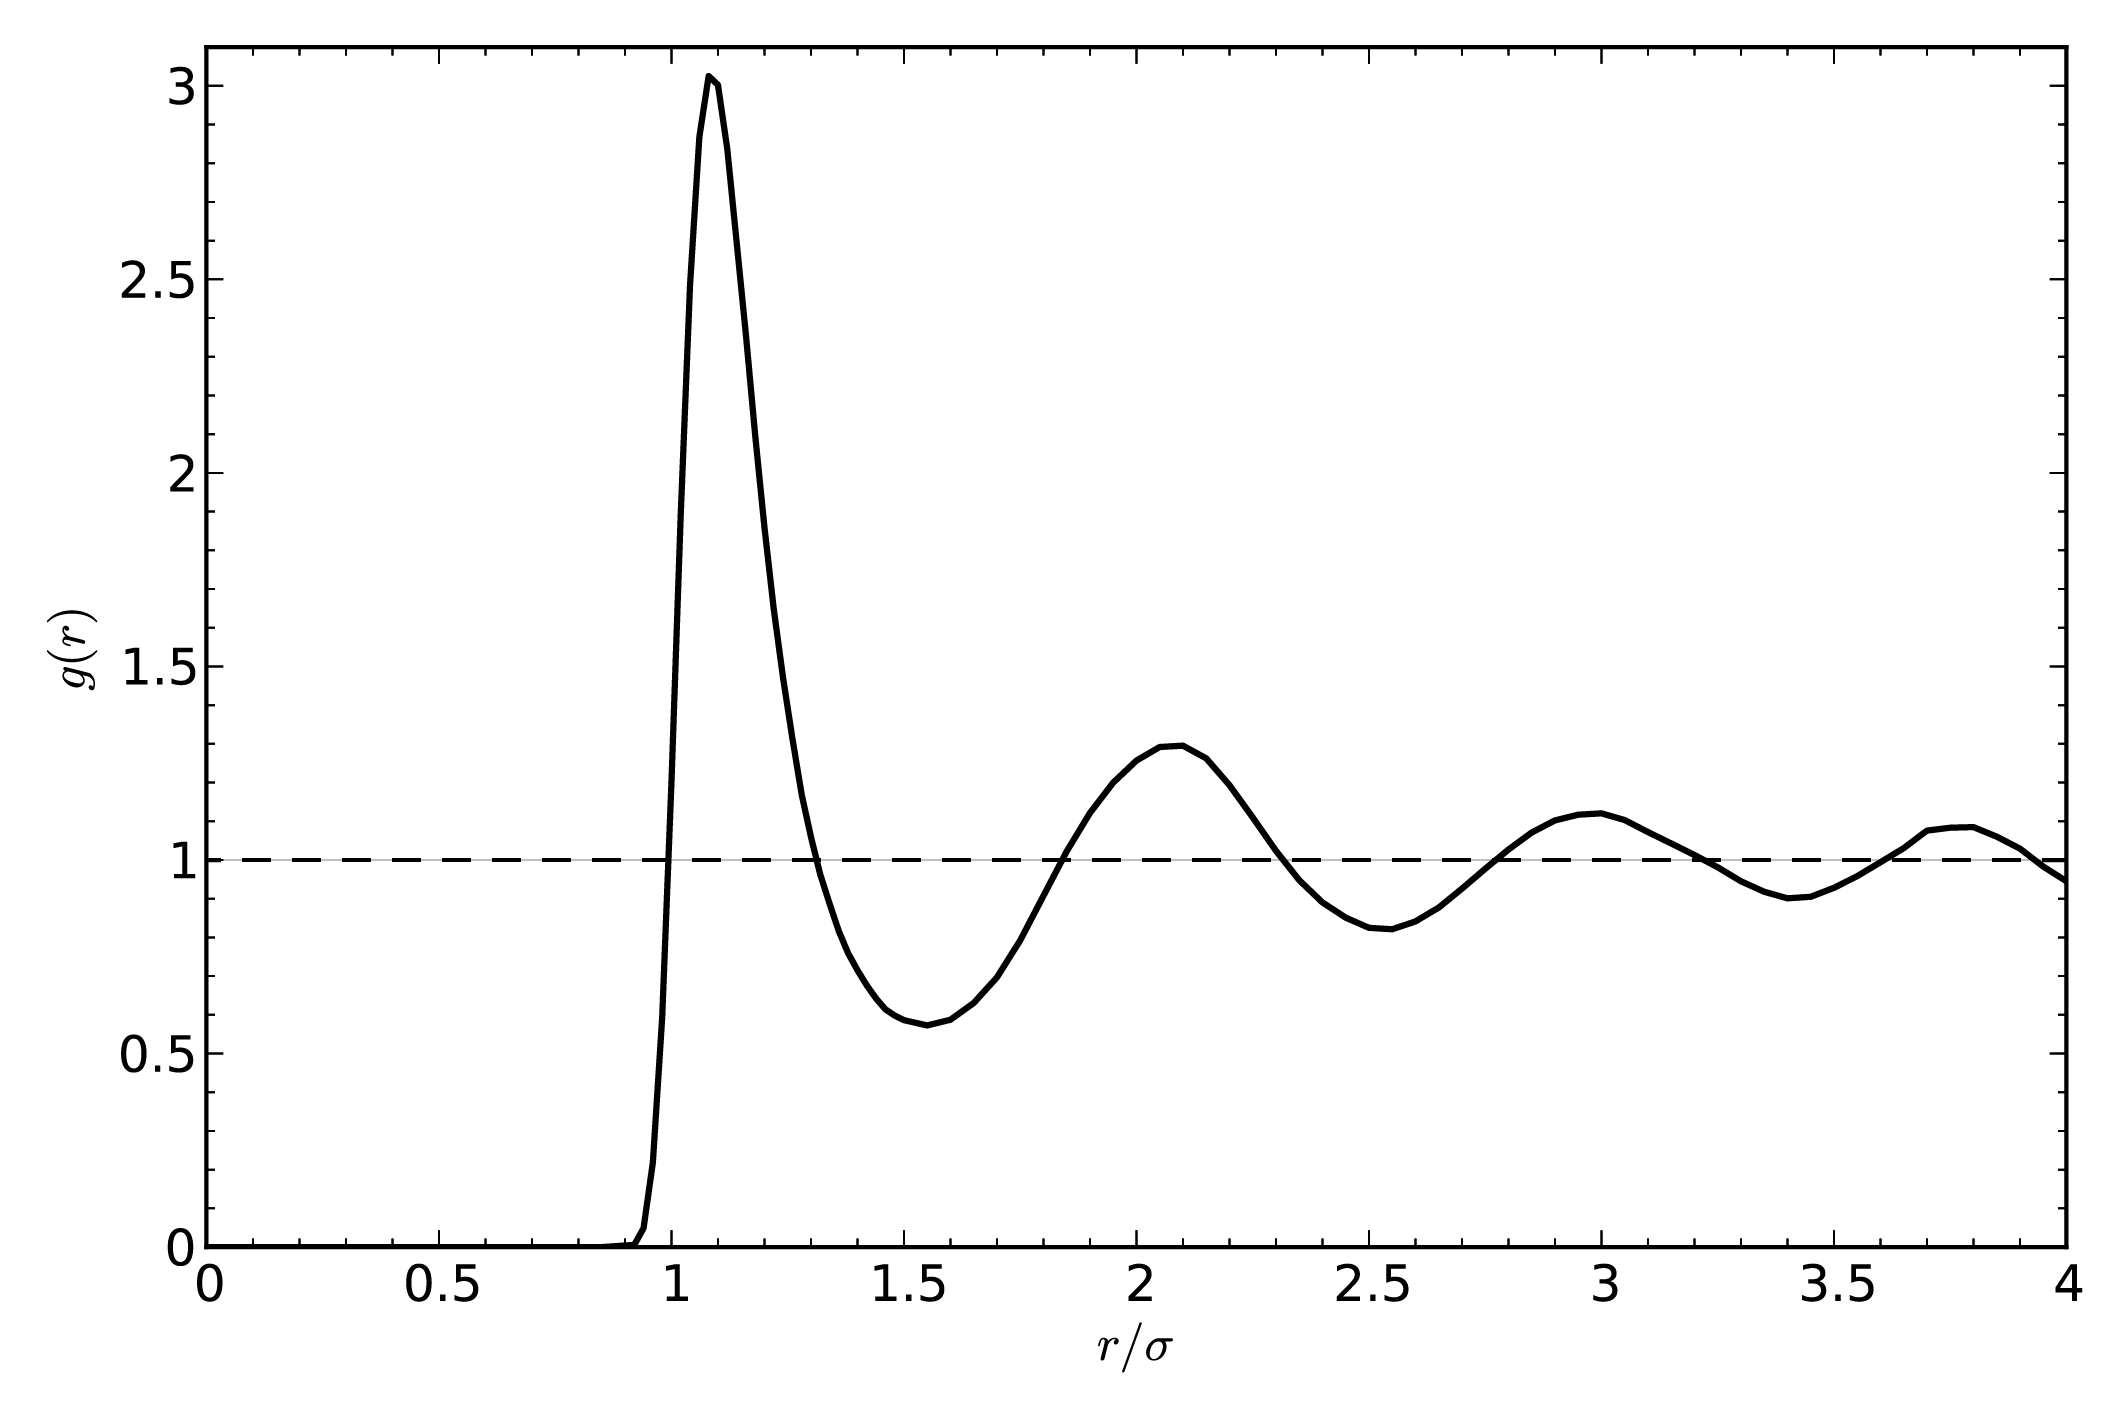
\includegraphics[width=\textwidth, trim=0cm 0cm 0cm 0cm, clip]{MD/figures/lennardjonesg_of_r.png}}
\label{fig:fcc_lattice_g_of_r}
\centering
\caption{The radial distribution function of an FCC lattice. The first peak reveals the distance between the face atoms and the corner atoms. Source: \url{http://en.wikipedia.org/wiki/Radial_distribution_function}.}
\end{figure}
The radial distribution function is defined as
\begin{align}
    \label{eq:g_of_r}
    g(r)dr &= \left\langle \sum_{i\neq j}\delta(r - |\vec r_i - \vec r_j|)\right\rangle{V\over N(N-1)4\pi r^2}\\
    &= {1 \over N} \left\langle \sum_{i\neq j}\delta(r - |\vec r_i - \vec r_j|)\right\rangle
\end{align}
where $N$ is seen as a normalization factor making sure that $\lim r\rightarrow \infty = 1$. A numerical implementation would loop over all relevant atom pairs, calculate their relative distance $r_{ij}$ and create a histogram over such distances. We would have to normalize each histogram bin by the volume of spherical shell as in \eqref{eq:g_of_r} with $dr\rightarrow \Delta r$ since each bin has a radial thickness. An implementation in $c++$ is given in  listing \ref{lst:g_of_r}.

\begin{lstlisting}[caption=Calculation of $g(r)$., label=lst:g_of_r]
vector<double> calculate_g_of_r(System &system, int num_bins) {
    // Create empty array of num_bins bins to store g(r)
    vector<double> g_of_r(num_bins,0);
    int num_atoms = system.r.size();

    // Loop over all atom pairs and put their distance into bin
    for(int i=0; i<num_atoms-1; i++) {
        Vector3D &r1 = system.r[i];
        for(int j=i+1; j<num_atoms; j++) {
            Vector3D &r2 = system.r[j];
            double dr = (r1 - r2).length();
            int bin_index = (dr / r_max) * num_bins;
            g_of_r[bin_index]++;
        }
    }

    // Normalize each bin
    for(int bin_index=0; bin_index<num_bins; bin_index++) {
        double r_inner = r_max * double(bin_index) / num_bins;
        double r_outer = r_max * double(bin_index+1) / num_bins;
        double r = 0.5*(r_inner + r_outer);
        double dr = r_outer - r_inner;

        double shell_volume = 4*M_PI*pow(r,2.0)*dr;
        double density = num_atoms/system.volume;
        g_of_r[bin_index] /= shell_volume * (num_atoms-1) * density;
    }

    return g_of_r;
}
\end{lstlisting}
The example code has complexity $N^2/2$, but since $g(r)$ is interesting only for relatively small $r$, we can improve the algorithm substantially by creating neighbor lists for each atom before looping over all relevant pairs. Experimentally, it is possible to measure the radial distribution function through diffraction experiments. By firing a beam of electrons or neutrons at the crystal, the electrons will be diffracted in different directions depending on the crystallic structure. One can measure the angles and intensities of the diffracted beams and then measure what is called \textit{structure factor} given by
\begin{align}
    S(\vec q) = {1\over N}\left\langle \sum_{jk} e^{-i\vec q(\vec R_j - \vec R_i)}\right \rangle,
\end{align}
where $\vec q$ is the spatial frequency (reciprocal coordinate), $N$ the number of atoms and $\vec R_{ij}$ the position of particles $i$ and $j$ respectively. We will not go into more detail in what the structure factor is other than that it is related to $g(r)$ through
\begin{align}
    S(q) = 1 + 4\pi\rho_n\frac{1}{q}\int dr r\sin(qr)[g(r) - 1],
\end{align}
if we assume that the material is isotropic\cite{kittel1996introduction}. The $g(r)$ can then be found through the inverse fourier transform
\begin{align}
    g(r) = 1 + {1\over 2\pi^2\rho_n r} \int dq(S(q) - 1)q\sin(qr).
\end{align}

\section{Diffusion constant}
The diffusion constant $D$ is defined by using the Einstein relation
\begin{align}
    \langle \Delta r^2 \rangle = 2dDt,
\end{align}
where $t$ is time, $d$ is the number of spatial dimensions and $\langle \Delta r^2 \rangle$ is average square displacement 
\begin{align}
    \langle \Delta r^2 \rangle = {1 \over N} \sum_{n=1}^N |\vec r(t) - \vec r(0)|^2.
\end{align}
In three dimensions, the diffusion constant is then found as
\begin{align}
    D = {\langle \Delta r^2 \rangle\over 6t}.
\end{align}
This is a fairly simple calculation, but in the MD-simulation, we need to keep track of how far each atom has moved from its initial position. A simple implementation is given in listing \ref{lst:diffusion}.
\begin{lstlisting}[caption=Calculation of the diffusion constant., label=lst:diffusion]
double calculate_diffusion_constant(System &system) {
    double rSquared = 0;
    for(int atom_index=0; atom_index<system.num_atoms; atom_index++) {
        double dr2 = (system.r[atom_index] - system.r0[atom_index]).length_squared();
        rSquared += dr2;
    }
    rSquared /= system.num_atoms; // Normalize to get <r^2>
    double diffusion_constant = rSquared / (6*system.t);
    return diffusion_constant;
}
\end{lstlisting}
